\documentclass[12pt,letterpaper]{article}
\usepackage{graphicx,textcomp}
\usepackage{natbib}
\usepackage{setspace}
\usepackage{fullpage}
\usepackage{color}
\usepackage[reqno]{amsmath}
\usepackage{amsthm}
\usepackage{fancyvrb}
\usepackage{amssymb,enumerate}
\usepackage[all]{xy}
\usepackage{endnotes}
\usepackage{lscape}
\newtheorem{com}{Comment}
\usepackage{float}
\usepackage{hyperref}
\newtheorem{lem} {Lemma}
\newtheorem{prop}{Proposition}
\newtheorem{thm}{Theorem}
\newtheorem{defn}{Definition}
\newtheorem{cor}{Corollary}
\newtheorem{obs}{Observation}
\usepackage[compact]{titlesec}
\usepackage{dcolumn}
\usepackage{tikz}
\usetikzlibrary{arrows}
\usepackage{multirow}
\usepackage{xcolor}
\newcolumntype{.}{D{.}{.}{-1}}
\newcolumntype{d}[1]{D{.}{.}{#1}}
\definecolor{light-gray}{gray}{0.65}
\usepackage{url}
\usepackage{listings}
\usepackage{color}

\definecolor{codegreen}{rgb}{0,0.6,0}
\definecolor{codegray}{rgb}{0.5,0.5,0.5}
\definecolor{codepurple}{rgb}{0.58,0,0.82}
\definecolor{backcolour}{rgb}{0.95,0.95,0.92}

\lstdefinestyle{mystyle}{
	backgroundcolor=\color{backcolour},   
	commentstyle=\color{codegreen},
	keywordstyle=\color{magenta},
	numberstyle=\tiny\color{codegray},
	stringstyle=\color{codepurple},
	basicstyle=\footnotesize,
	breakatwhitespace=false,         
	breaklines=true,                 
	captionpos=b,                    
	keepspaces=true,                 
	numbers=left,                    
	numbersep=5pt,                  
	showspaces=false,                
	showstringspaces=false,
	showtabs=false,                  
	tabsize=2
}
\lstset{style=mystyle}
\newcommand{\Sref}[1]{Section~\ref{#1}}
\newtheorem{hyp}{Hypothesis}

\title{Problem Set 5}
\date{Vanessa Wong}
\author{QTM 200: Applied Regression Analysis}

\begin{document}
	\maketitle
	
	\section*{Instructions}
	\begin{itemize}
		\item Please show your work! You may lose points by simply writing in the answer. If the problem requires you to execute commands in \texttt{R}, please include the code you used to get your answers. Please also include the \texttt{.R} file that contains your code. If you are not sure if work needs to be shown for a particular problem, please ask.
		\item Your homework should be submitted electronically on the course GitHub page in \texttt{.pdf} form.
		\item This problem set is due at the beginning of class on Wednesday, March 4, 2020. No late assignments will be accepted.
		\item Total available points for this homework is 100.
	\end{itemize}
	
		\vspace{.5cm}
	
\noindent  Using the \texttt{teengamb} dataset, fit a model with \texttt{gamble} as the response and the other variables as predictors. 

\vspace{.5cm}
\lstinputlisting[language=R, firstline=41, lastline=43]{PS5.R}  
\vspace{.5cm}
Answer the following questions:
\vspace{.5cm}
\begin{enumerate}[(a)]
	 \item Check the constant variance assumption for the errors by plotting the residuals versus the fitted values. 
	 \lstinputlisting[firstline=49, lastline=51]{PS5.R}
	 \item [-] After fitted value (y hat) equals ~ 45, variance seems to increase/residuals deviate more from 0. variance does not appear to be constant.
	 	\item [-]
	 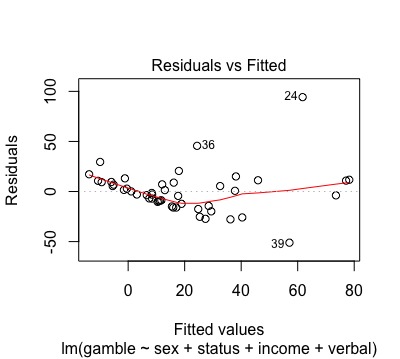
\includegraphics[width=7cm]{residual.png}
	\item Check the normality assumption with a Q-Q plot of the studentized residuals. 
	\lstinputlisting[firstline=54, lastline=55]{PS5.R}
	\item[-] The normality assumption appears to be met because almost all points are very tightly clustered along the QQ line.
		\item [-]
	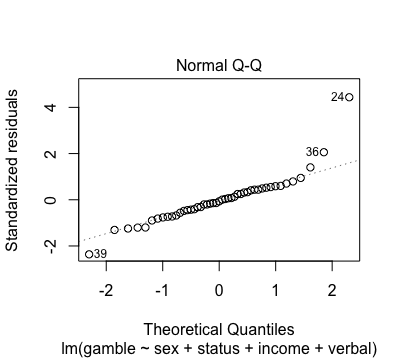
\includegraphics[width=7cm]{Qqplotps5.png}
	\item Check for large leverage points by plotting the $h$ values.
	\lstinputlisting[firstline=58, lastline=62]{PS5.R}
	\item[-] Using the average hat value as a threshold (thresholds = 2 * hbar and 3 * hbar), there are 4 high leverage points in this dataset: observations 31, 33, 35, and 42. These four points have are potentially influential i.e. have the potential to greatly affect the regression model.
	\item [-]
	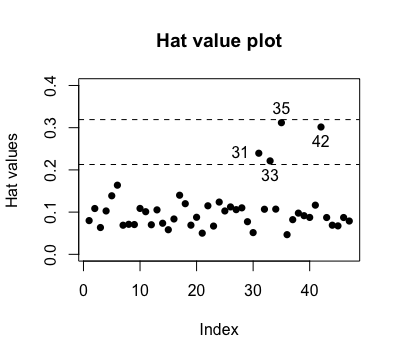
\includegraphics[width=7cm]{Hatvalueplot.png}
	\item Check for outliers by running an \texttt{outlierTest}. \lstinputlisting[firstline=67, lastline=67]{PS5.R}
	\item [-] According to outlier test, observation 24 has an adjusted (Bonferroni) p-value ~ 0. therefore, observation 24 is an extreme residual in this model.
	\item Check for influential points by creating a "Bubble plot" with the hat-values and studentized residuals.
	\lstinputlisting[firstline=71, lastline=76]{PS5.R}
	\item [-] Observations 31, 33, 35, and 42 are influential points because all 4 are above at least one threshold for studentized residuals and hat values. This means all 4 points are both high leverage and are regression outliers, making them influential points (they greatly affect the regression model).Observation 24 was also identified because while it did not pass any of the hat value thresholds, it has an unusally large Cook's distance.
		\item [-]
	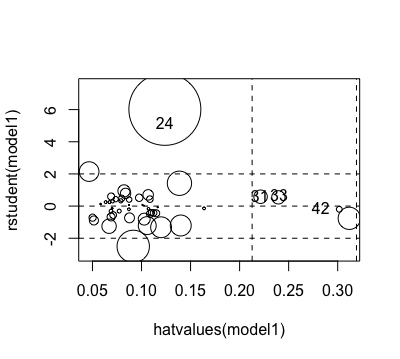
\includegraphics[width=7cm]{Bubble.png}
	% \item N/A.
\end{enumerate}

\lstinputlisting{PS5.R}

\end{document}
